\documentclass[a0,portrait]{a0poster}
\usepackage{graphicx}
\usepackage{multicol}
\usepackage{times}
\usepackage{color}
\usepackage[utf8]{inputenc}
\usepackage{amsmath}
\usepackage{caption}
\usepackage{enumitem}
\usepackage{booktabs}
\usepackage{xcolor}
\usepackage{parskip}          % Activa el paquete para controlar el espacio entre párrafos
\usepackage{comment} %sirve para agregar comentarios en mas de una línea del código

\definecolor{miRojo}{rgb}{0.82, 0.32, 0.31}  % Definir el color usando valores rgb
\definecolor{lightgray}{gray}{0.9}  % Color gris claro para subrayado
\definecolor{miGray}{gray}{.6}  % Color gris claro para subrayado
\definecolor{miVerde}{rgb}{0.0, 0.6, 0.0}  % Definir un color verde personalizado
\setlength{\parindent}{2em}   % Ajusta la sangría global
\setlength{\parskip}{2em}     % Ajusta el espacio entre párrafos

\setlength{\columnsep}{2cm}
\setlength{\columnseprule}{2.5pt}
\def\columnseprulecolor{\color{miRojo}}

% Crear comando para secciones subrayadas y centradas
\newcommand{\customsection}[1]{
    \begin{center}
        %\color{miRojo}
        \vspace{1cm} % Espacio entre el parrafo anterior y el subtitulo
        %\rule{15cm}{7.5pt} % Línea de 5cm de largo y 2.5pt de grosor
        \color{black}
        \textbf{\Huge #1}
        \color{miRojo}
        \vspace{.5cm} % Es pacio entre el título y la línea
        %\rule{15cm}{7.5pt} % Línea de 5cm de largo y 2.5pt de grosor
        \hrule height 2.5pt  % Línea subrayada gris
        \vspace{.5cm} % Espacio después de la línea
    \end{center}
}

\begin{document}
% Recuadro inicial en todo el ancho de la hoja sin márgenes
\noindent
\fcolorbox{miGray}{miGray}{%
    \hspace{0pt} % Eliminar márgenes extras
    \makebox[.984\linewidth]{ % Asegurar que ocupe todo el ancho
        \begin{minipage}{\linewidth}
            % Cabecera con el logo alineado a la izquierda
            \begin{center}
                
\includegraphics[width=.3\linewidth]{logo_fae_web.png}\\
                \vspace{-3.5cm} % Ajusta este valor si es necesario para el espaciado
                \VeryHuge \textbf{\emph{Evaluación del poder predictivo de estrategias técnicas de tendencia y momentum sobre acciones americanas}}\par
                \vspace{1cm}
                \Huge Mateo Canales Briceño, Cristóbal González Araya, Tomás Leyton Muñoz \par
                \huge Escuela de Ingeniería Comercial, Universidad Diego Portales, 2024 \par
                \vspace{1cm}
            \end{center}
        \end{minipage}%
    } % Fin de makebox
} % Fin del inicial


\vspace{2cm}
\normalsize %tamaño de la letra, recomiendo Large
\begin{multicols}{2}

    % Sección 1: Resumen
    \customsection{Resumen}
    \par
     Esta tesis evalúa el poder predictivo de estrategias técnicas de tendencia y momentum sobre el mercado de acciones americanas. Utilizando indicadores como SMA y EMA, se implementaron modelos econométricos para predecir la dirección de las acciones en el índice SyP500. Los resultados sugieren que al menos la mitad de los indicadores son significativos, lo que valida el uso de estas estrategias en la toma de decisiones de inversión.
    % Sección 2: Introducción
    \customsection{Introducción}
    \par
     En las últimas décadas, el mercado de acciones de EE. UU. ha experimentado cambios significativos, lo que ha llevado al desarrollo de estrategias técnicas como tendencia y momentum. Estas estrategias, basadas en análisis de datos históricos, son herramientas clave para predecir movimientos futuros en los precios de las acciones.
    % Sección 3: Metodología
    \customsection{Metodología}
    \par
    \textbf{Datos:} Se utilizó una base de datos que abarca desde enero de 2019 hasta diciembre de 2023, con precios de cierre diarios obtenidos de Yahoo Finance. 
    \par
    \textbf{Modelos Econométricos:} Se construyeron varios modelos de regresión lineal para evaluar la capacidad predictiva de los indicadores técnicos. Las regresiones se estimaron con HAC según Newey-West (1987).
    
    La ecuación general del modelo de regresión utilizado es la siguiente:

    \begin{equation}
        R_t = \alpha + \beta_1 \cdot SMA_t + \beta_2 \cdot EMA_t + \beta_3 \cdot MACD_t + \varepsilon_t
    \end{equation}
    
    Donde:
    \begin{itemize}
        \item $R_t$ es el retorno en el tiempo $t$.
        \item $SMA_t$ es la media móvil simple en el tiempo $t$.
        \item $EMA_t$ es la media móvil exponencial en el tiempo $t$.
        \item $MACD_t$ es el indicador MACD en el tiempo $t$.
        \item $\alpha$ es la intersección.
        \item $\beta_1$, $\beta_2$, y $\beta_3$ son los coeficientes estimados.
        \item $\varepsilon_t$ es el término de error en el tiempo $t$.
    \end{itemize}
    \columnbreak
    \par
    \textbf{Indicadores Técnicos:}
    \begin{itemize}
        \item SMA:(1,50);(1,150);(1,200);(5,200).
        \item MACD2:(12,26,9).
        \item ROC:(10);(50);(200).
        \item RSI:(14);(20);(50).
        \item WLPR:(14);(20);(50).
    \end{itemize}
    % Sección 4:Resultados
    \customsection{Resultados}
    \par  
    Aquí debería ir unas cuantas tablas de varias weas raras para explicar un poco las cagás que estamos viendo 
    \vspace{2cm}
    
    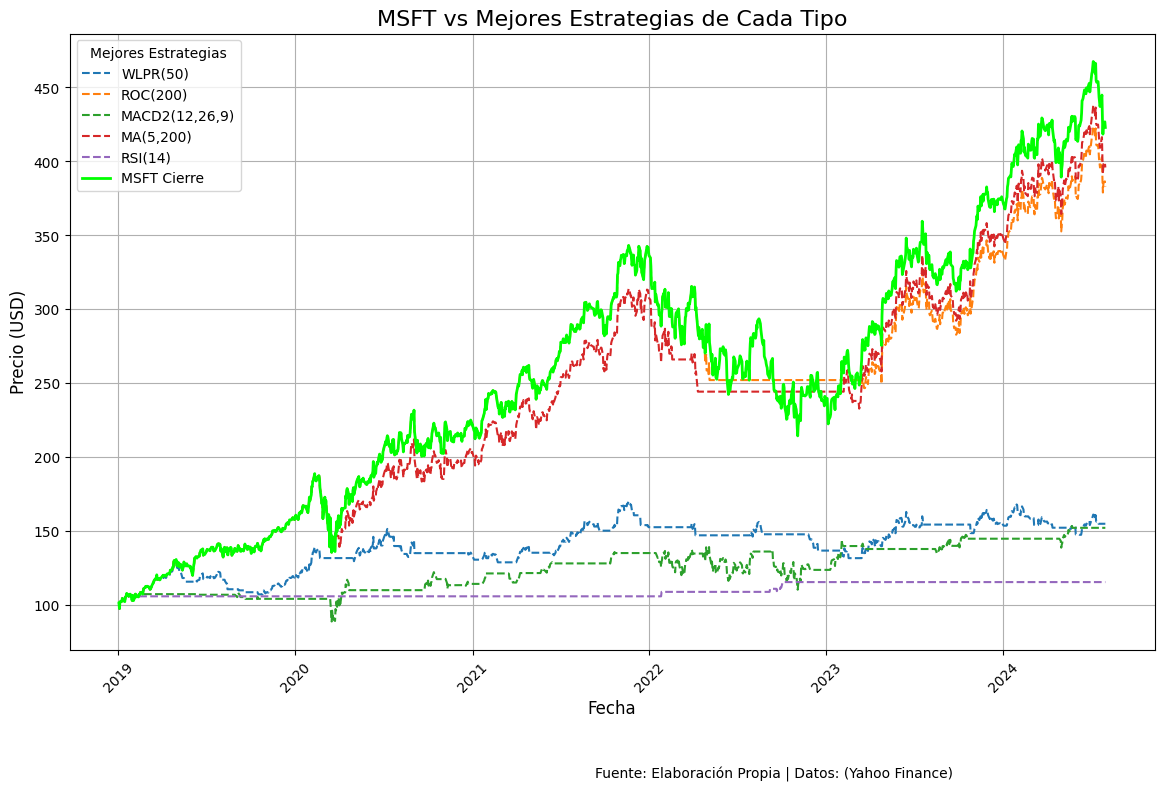
\includegraphics[width=0.9\linewidth]{grafico_mejores_estrategias_MSFT.png}
    \captionof{figure}{Ejemplo de gráfico de resultados.}
    % Sección 5: Conclusiones
    \customsection{Conclusiones}
    \par
    \indent La investigación valida el uso de estrategias de tendencia y momentum para predecir el mercado de acciones estadounidense. Estas herramientas son valiosas para los inversores que buscan optimizar su toma de decisiones en un entorno bursátil dinámico. 
    % Sección 6: Referencias   
    \customsection{Referencias}
    \par
         \begin{itemize}
            \item Subrahmanyam, A. (2018). Equity market momentum: A synthesis of the literature and suggestions for future work.
            \item Jegadeesh, N., y Titman, S. (1993). Returns to buying winners and selling losers: Implications for stock market efficiency.
            \item Lim, B. Y., Wang, J. G., y Yao, Y. (2018). Time-Series Momentum in nearly 100 years of stock returns.            \item Paper 4
            \item Paper 5
        \end{itemize}
        
    
    
    
    
\end{multicols}
\end{document}
